\chapter{Logkorrelation in Cloud-Umgebungen}\label{02_jcorrelat}
\thispagestyle{fancy}

Im folgenden Kapitel wird eine Forschungsarbeit der Fachhochschule Fulda 
\cite{reissmann} vorgestellt. Ziel der Forschung war und ist es, ein gut skalierendes 
System zu entwickeln um eine automatisierte Auswertung von Syslog-Meldungen in 
Cloud-Umgebungen bereit zu stellen. Aufgrund der enormen Datenmengen die in solchen 
Umgebungen anfallen kann eine Auswertung nur mittels korrelations- und 
Aggregationsverfahren geschehen. Um dieses Ziel zu erreichen kommen verschiedene 
Standards und eine Reihe von Software-Lösungen zum Einsatz.

Nachfolgend werden einige wichtige Begriffe geklärt, die Anforderungen identifiziert, die 
verwendeten Standards und die eingesetzte Software erläutert und im Weiteren Verlauf des 
Abschnitts wird anhand eines Beispiels eine Syslog-Korrelation vorgenommen.

\section{Anforderungen}\label{anforderungen}

Viele Unternehmen haben in den letzten Jahren einen großen Teil ihrer IT-Infrastruktur 
ausgelagert. Laut Analysen werden bis 2025 80 \% aller Unternehmen \cite{web_ix} 
weltweit ihre eigene Rechenzentrumsinfrastruktur abgeschaltet haben. Die wenigen Anbieter 
von Cloud-Lösungen stehen in Konkurrenz miteinander, daher existieren auch keine 
einheitlichen Schnittstellen um auf die Cloud-Konfigurationen zuzugreifen. Für die 
Überwachung, speziell von Sicherheitskritischen Ereignissen, stehen ebenso nur 
proprietäre Schnittstellen jedes Anbieters zur Verfügung. Aus diesem Grund soll ein 
System geschaffen werden, das die gewaltige Menge an aufkommenden Logdaten, unabhängig 
vom Anbieter, analysiert und sicherheitskritische Ereignisse unverzüglich 
erkennt. Insbesondere soll das System das dynamisch sinkende und wachsende 
Syslog-Aufkommen beherrschen können. Denn durch die fluide Kostenstruktur der 
Cloud-Anbieter können schnell neue virtuelle Maschinen erstellt und entfernt werden, je 
nachdem wie viel Leistung der Kunde gerade benötigt.
Darüber hinaus sollen Meldungen auch persistent gespeichert werden, vornehmlich zur 
Erstellung von Trends und Langzeitanalysen, dabei soll der benötigte Speicherplatz so 
gering wie möglich gehalten werden.

\section{Beispielszenario}\label{szenario}

Im weiteren Verlauf dieses Kapitels soll zur detaillierteren Darstellung der 
Leistungsfähigkeit einer automatischen Syslog-Korrelation ein gängiges 
Angriffsszenario dienen. Eine \textit{ssh}-BruteForce Attacke auf eine beliebige Anzahl
an überwachten Systemen. Dabei soll genau der eine erfolgreiche Login innerhalb  der 
enormen Anzahl an erfolglosen oder ungültigen Versuchen identifiziert werden. Dieses 
recht einfache Szenario ist bei der erheblichen Anzahl an möglichen Systemen (10K+) 
manuell unmöglich zu bewerkstelligen.

\newpage
\section{JCorrelat}\label{sec_jcorrelat}

In Abbildung \ref{pic:jcorrelat} \cite[47]{reissmann} ist der schematische Aufbau von 
JCorrelat dargestellt, ein Prototyp der die Anforderungen aus Abschnitt 
\ref{anforderungen} erfüllen soll. Die hinzugefügten Nummern dienen der Übersichtlichkeit 
im weiteren Erklärungsverlauf.   

\begin{figure}[htbp]
    \caption{Aufbau von JCorrelat}
    \label{pic:jcorrelat}\vspace{0.2cm}
    \centering
    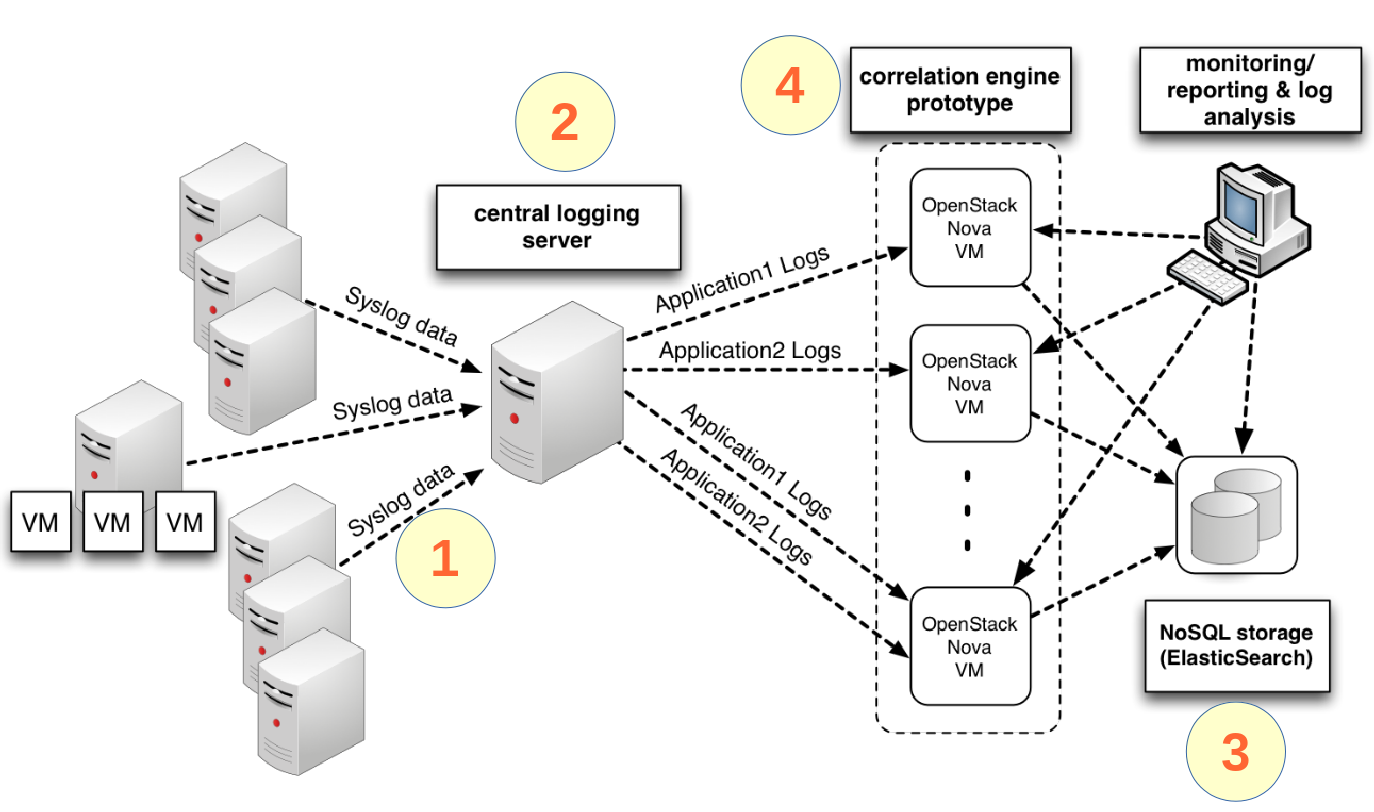
\includegraphics[scale=0.36]{img/schema-correlat}
    
\end{figure}

\subsection{Syslog-Protokoll} \label{syslog-proto}

Als Ereignisquelle und als Grundlage für neu generierte Meldungen wird das 
Syslog-Protokoll verwendet. Es ist das meist verbreitete Log-Format und wurde 
bereits in RFC 3164 standardisiert, jedoch sieht dieser Standard keine strukturierten 
Daten (\texttt{key $\Rightarrow$ value}) innerhalb einer Syslog-Nachricht vor. 
Erst mit RFC 5424 \cite{rfc5424} wurde diese Funktionalität hinzugefügt.

\begin{table}[ht]
    \caption{Aufbau RFC 5424}
    \label{table:rfc5424}\vspace{0.2cm}
    \centering{
        \renewcommand{\arraystretch}{1.3}
    \begin{tabular}{|l|c|c|}
        \hline 
        \rowcolor{gray!40} \textbf{Feld}&  \textbf{Inhalt}& \textbf{Beispiel}\\ 
        \hline
        \hline
         \multicolumn{3}{|l|}{\cellcolor{shadecolor}\textbf{HEADER}}\\
         \hline
         facility & $int \in \{0..23\}$  & $<$\textbf{16}5$>$ (\texttt{local0}) \\ 
        \hline 
        \rowcolor{green!15} severity & $ int \in \{0..7\}$  &$<$16\textbf{5}$>$  
        (\texttt{Notice})\\ 
        \hline
         timestamp & \texttt{RFC3339}  &\verb|2003-10-11T22:14:15.003Z|\\ 
        \hline 
         hostname & string  &\verb|mymachine.example.com|\\ 
        \hline 
        \rowcolor{green!15} tag &string  &\verb|evntslog|\\
        \hline
         \multicolumn{3}{|l|}{\cellcolor{shadecolor}\textbf{MESSAGE}}\\     
        \hline
         MSGID& string &\verb|ID47| \\
        \hline
        \rowcolor{green!15} structured data& key=value &\verb|eventID="1011"| \\
        \hline
         content &string&\verb|An application event log...| \\
        \hline
    \end{tabular} 
    }
\end{table}

\newpage

\begin{figure}[h]
    \caption{Beispiel RFC5424 Syslog-Meldung}
    \label{log_example}\vspace{0.2cm}
    \centering
    \begin{shaded*}
    \small{
        \begin{verbatim}
        
        
        <165> 2003-10-11T22:14:15.003Z mymachine.example.com evntslog - ID47 
        [exampleSDID@32473 iut="3" eventSource="Application" eventID="1011"] BOMAn 
        application event log entry...
        \end{verbatim}}
    \end{shaded*}
\end{figure}

Tabelle \ref{table:rfc5424} zeigt den Aufbau eines Syslog-Paketes nach RFC 5424 und 
Abbildung \ref{log_example} die dazugehörige RFC 5424 konforme Nachricht. Die für 
die weitere Verwendung wichtigsten Felder wurden grün markiert. Dazu zählt der 
Schweregrad (\textit{severity}), wobei 0 (\texttt{Emergency}) den höchsten und 7 
(\texttt{DEBUG}) den niedrigsten Schweregrad darstellt. Das \textit{tag}-Feld, das zum 
Beispiel die Herkunft (Programm) und die zugehörige \textit{process ID} beinhalten kann. 
Am wichtigsten ist das \textit{structured data}-Feld, welches mit beliebigen 
strukturierten Daten versehen werden darf.

\subsection{Normalisierung von Syslog-Meldungen}\label{syslog-konsolidierung}

Diese Sektion erläutert Punkt \textbf{2} in Abbildung \ref{pic:jcorrelat}, es handelt 
sich um den zentralen Syslog-Server. Als Software kommt die Open Source - Lösung 
\textit{rsyslog}\footnote{\url{https://rsyslog.com}} zum Einsatz. \textit{rsyslog} ist 
RFC 5424 konform, äußerst performant und durch Module erweiterbar. Eben eines dieser 
Module kommt auch im hier vorgestellten Korrelationssystem zum Einsatz: 
\textit{liblognorm}, mittlerweile ein fester Bestandteil von \textit{rsyslog}.\\ 

Alle Applikationen senden ihre Syslog-Meldungen an diesen Server und damit auch alle 
SSH-Dienste. Somit passieren alle Syslog-Nachrichten über einen erfolgreichen, 
fehlgeschlagenen oder ungültigen Login dieses System. In Abbildung \ref{ssh_example} wird 
jeweils ein Beispiel pro Fall abgebildet.

\begin{figure}[h]
    \caption{Beispiele SSH-Meldungen}
    \label{ssh_example}\vspace{0.2cm}
    \centering
    \begin{shaded*}
    \small{      
        \begin{verbatim}        


Jan 29 16:00:25 HOST sshd[2039]: Accepted password for root from 10.0.23.4 port 39110 ssh2
        
Jan 29 16:06:00 HOST sshd[2032]: Failed password for root from 10.0.23.4 port 54548 ssh2

Jan 29 16:08:39 HOST sshd[2023]: Failed password for invalid user test from 10.0.23.4 
port 57165 ssh2
\end{verbatim}}
\end{shaded*}
\end{figure}

\textit{liblognorm} ist nun in der Lage diese Meldungen auf Basis vorher definierter 
Regeln zu durchsuchen (für das konkrete Beispiel finden sich die Regeln im Anhang unter 
Abbildung \ref{app:liblognorm-rule}) und die relevanten Informationen zu extrahieren.  
Aus diesen Daten generiert \textit{liblognorm} eine neue Syslog-Meldung in dem es aus den 
aufgeschlüsselten Feldern Protokoll, Nutzername, Port und Quelladresse strukturierte 
Daten bildet (Anhang: Abbildung \ref{app:liblognorm-normalisation}). Zusätzlich wird die 
neue Meldung mit einem neuen \textit{syslog-tag} names \texttt{SSHFAILURE} oder 
\texttt{SSHSUCCESS} versehen und an die Korrelationsinstanz weitergeleitet.\\

\textit{liblognorm} normalisiert und serialisiert Daten, die aus verschiedenen Quellen 
stammen und unterschiedlich kodiert sein können zu neuen Nachrichten. Damit werden 
Redundanzen aus den Meldungen entfernt und eindeutige \textit{syslog-tags} zu schnelleren 
Identifizierung durch die Korrelationsinstanz gesetzt. 


\newpage

\subsection{Korrelation von Syslog-Meldungen}\label{syslog-korrelation}

Mithilfe der normalisierten Meldungen wird nun versucht ein Zusammenhang zwischen den 
Syslog-Ereignissen zu erkennen. Diese Ereigniskorrelation ist der rechenaufwändigste 
Schritt und kann daher, wie in Punkt \textbf{3} in Abbildung \ref{pic:jcorrelat} zu 
erkennen ist, auf mehrere virtuelle Systeme verteilt werden.\\

Die Korrelation der Syslog-Meldungen durch \textit{JCorrelat} erfolgt mithilfe von 
\textit{Drools-Fusion}\footnote{\url{https://www.drools.org/}}. \textit{Drools-Fusion} 
ist eine \textit{complex event processing engine}, mit dessen Hilfe zeitliche 
Schlussfolgerungen gezogen werden können. Um dieses Ziel zu erreichen werden Regeln 
erstellt um Events zu beschreiben und alle Nachrichten die zu einer Regel 
gehören werden analysiert, die restlichen Meldungen werden verworfen. Findet sich eine 
zeitliche Übereinstimmung, wird der Event ausgelöst, die 
Nachricht wird mit einem \textit{syslog-tag} versehen und zur weiteren Analyse und 
Speicherung  weitergeleitet. \textit{Drools-Fusion} behält dazu alle relevanten 
Syslog-Meldungen in einer \textit{in memory engine} vor und verwendet das Prinzip der 
\textit{sliding windows} um Zusammenhänge zu erkennen. Abbildung \ref{pic:drools} 
\cite[70]{drools-slide} demonstriert die Funktionsweise der \textit{sliding-windows}, ein 
Quader ist im hier verwendeten Beispiel eine relevante Syslog-Meldung, die Fenster 
analysieren immer eine gewisse Anzahl an Meldungen aus verschiedenen Quellen, die in 
einem bestimmtem Zeitfenster erzeugt wurden. Erfüllt das \textit{joined-window} dann den 
Bedingungen in der definierten Regel, kann ein Event ausgelöst werden.    

\begin{figure}[htbp]
    \caption{\textit{sliding window}-Prinzip}
    \label{pic:drools}\vspace{0.2cm}
    \centering
    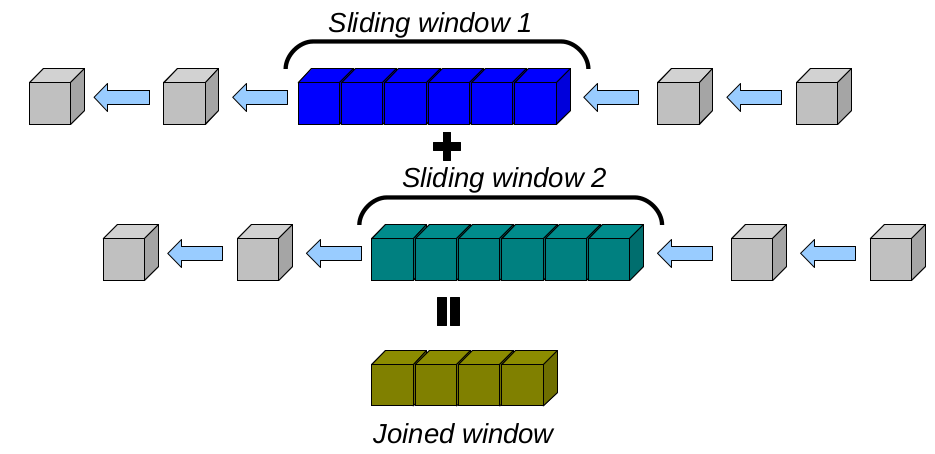
\includegraphics[scale=0.36]{img/drools-slide-00}
    
\end{figure}

Um nun, wie in Abschnitt \ref{szenario} beschrieben, einen erfolgreichen SSH Brute-Force 
Angriff zu erkennen, muss zuerst eine Brute-Force-Attacke erkannt werden, dazu dient die 
Regel \texttt{SSH brute-force attempt} (Anhang: \ref{app:drools-warning}). Die Regel 
untersucht nur Syslog-Meldungen die mit dem \textit{syslog-tag} \texttt{SSHFAILURE} 
versehen wurden. Es wird ein Event ausgelöst, wenn innerhalb von einer Minute vom 
gleichen Quell-Host und dessen verwendeten Benutzernamen 10 oder mehr fehlgeschlagene 
Login-versuche erfolgen. Als Event wird in diesem Fall eine neue Syslog-Meldung verfasst 
und mit dem Schweregrad \texttt{WARNING} und dem \textit{syslog-tag} \texttt{BRUTEFORCE} 
versehen. Die Meldung kann zum Beispiel persistent gespeichert werden (mehr dazu in 
Abschnitt \ref{nosql}) und an einen Monitor weitergeleitet werden.\\

Zur Erkennung einer erfolgreichen SSH Brute-Force-Attacke existiert ebenfalls eine 
beispielhafte Regel (Anhang: \ref{app:drools-emergency}). Die Regel \texttt{Successful 
SSH brute-force attack} löst einen Event aus, wenn innerhalb von 10 Sekunden nach dem 
Auftreten von Meldungen mit dem \textit{syslog-tag} \texttt{BRUTEFORCE} und 
\texttt{SSHFAILURE} und des zugehörigen Host und dessen verwendeten Benutzernamen, eine 
Meldung mit dem \textit{syslog-tag} \texttt{SSHSUCCSESS} auftritt, welche vom 
gleichen Host und aus der dazugehörigen Menge der Benutzernamen stammt.
Die generierte Syslog-Meldung wird mit dem gewichtigsten Schweregrad \texttt{EMERGENCY} 
und dem \textit{syslog-tag} \texttt{INCIDENT} markiert.\\

Mit diesem beiden Regeln ist es \textit{JCorrelat} unter der Zuhilfenahme von 
\textit{Drools-Fusion} möglich den einen erfolgreichen Login unter tausenden 
Loginversuchen innerhalb einer Brute-Force-Attacke zu identifizieren.

\subsection{persistente Speicherung}\label{nosql}

In diesem Abschnitt wird Punkt \textbf{4} aus Abbildung \ref{pic:jcorrelat} erläutert.\\

Neben der direkten Alarmierung von IT-Sicherheitskritischen Ereignissen, ist ein weiteres 
Ziel der IT-Sicherheit die Verfügbarkeit älterer Ereignisse, um auch über längere 
Zeiträume hinweg verbindlich Auskunft über den Zustand eines Systems zu geben oder die 
Daten mit neuen Methoden zu analysieren. Jedoch stellt die Speicherung von einer großen 
Menge sich ändernder Daten eine große Herausforderung dar. Mit \textit{JCorrelat} ist es 
möglich eine Vielzahl an Diensten zu überwachen, dabei können sich die zu betrachtenden 
Daten ständig ändern und Dienste können hinzukommen oder wegfallen.\\

Ein erster Ansatz wäre die Speicherung der normalisierten Daten (Abschnitt 
\ref{syslog-konsolidierung}) in einer relationalen Datenbank. Aufgrund der dynamischen 
Natur der Daten müsste für eine effiziente Verarbeitung das Schema einer solchen 
Datenbank stetig angepasst werden, dieser Aufwand ist enorm und nicht Zielführend.\\
Im Gegensatz zum relationalen Ansatz wird bei \textit{NoSQL}-Datenbanken (Not only SQL) 
kein oder nur ein minimales Schema gespeichert. Somit erlaubt dieses Konzept zu jeder 
Zeit eine Änderung der Datenstruktur. Darüber hinaus lassen sich 
\textit{NoSQL}-Datenbanken über viele Instanzen hinweg skalieren und liefern Daten sehr 
schnell aus. Allerdings mit den Nachteil, dass nicht auf allen Systemen zeitgleich die 
aktuellsten Daten zur Verfügung stehen.\\

Grundsätzlich lassen sich drei Konzepte von \textit{NoSQL}-Datenbanken identifizieren. 
Zuerst sind die einfachen \textbf{\emph{key-value}}-Implementierungen zu nennen, diese 
Datenbanken sind mit Abstand die schnellsten, da die Werte lediglich als \textit{BLOB} 
(Binary Large OBject) abgespeichert werden und somit nicht interpretiert werden. Damit 
sind die Werte nicht durchsuchbar, umso einfacher ist dafür die zugrunde liegende 
Programmierschnittstelle.\\

Die \textbf{\emph{column-oriented data stores}}-Lösungen speichern die Daten in Tabellen, 
ähnlich wie relationale-Lösungen, jedoch werden die Zeilen einer Tabelle in sogenannte 
shards (Scherben) unterteilt und die Spalten in Spaltengruppen, jeweils Abhängig von 
ihrem Schlüssel. Damit ist das Tabellenschema beliebig erweiterbar, aber eine 
Volltextsuche bietet diese Lösung nicht.\\

Davon abweichend arbeiten die \textbf{\emph{document-based data stores}}, sie speichern 
die Daten in \textit{documents} ab, welche eine Menge an beliebigen Objekten mit einer 
unterschiedlichen Anzahl an Attributen beschreiben. Objekte dürfen jederzeit neu 
angelegt werden und die Art und Anzahl ihrer \textit{key-value}-Paare ist nicht von 
Interesse. Als größter Vorteil ist bei diesem Konzept die Möglichkeit zur Volltextsuche 
zu nennen.\\

Aus den letztgenannten Gründen kommt bei \textit{JCorrelat} 
\textit{elasticsearch}\footnote{\url{https://www.elastic.co/products/elasticsearch}} zum 
Einsatz, was die Konzepte eines \textbf{\emph{document-based data stores}} umsetzt. 
\textit{JCorrelat} sendet die normalisierten und korrelierten Syslog-Meldungen für eine 
persistente Speicherung direkt an \textit{elasticsearch}. Monitoring- und 
Visualisierungssysteme können nun periodisch auf diese Daten zugreifen und kritische 
Ereignisse melden und visualisieren. Eine rudimentäre Visualisierung des SSH Brute-Force 
-Szenarios wurde in \cite{reissmann} veröffentlicht (Abbildung \ref{pic:logvis}). 
Alternative Möglichkeiten zu Visualisierung werden in Abschnitt \ref{ausblick} erläutert. 

\begin{figure}[htbp]
    \caption{Einfache Visualisierung durch JCorrelat}
    \label{pic:logvis}\vspace{0.2cm}
    \centering
    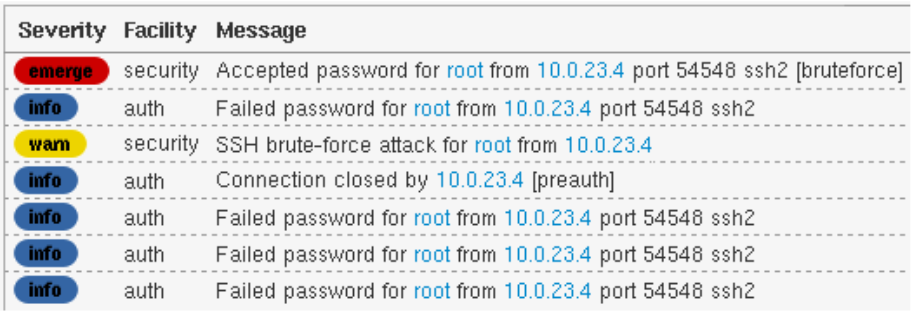
\includegraphics[scale=0.42]{img/correlat-ui}  
\end{figure}
\newpage
\subsection{Leistungsbetrachtung}\label{performance}

Wie schon in Sektion \ref{nosql} erwähnt, kostet das Korrelieren der Syslog-Meldungen am 
meisten Rechenzeit und ist daher der limitierende Faktor. Insbesondere stellt die 
Skalierbarkeit von \textit{Drools-Fusion} ein Problem dar, da es auf einer \textit{in 
memory engine} basiert, müssten mehrere Instanzen auf den gleichen Arbeitsspeicher 
zugreifen können (\textit{distributed memory}).
Jedoch existieren laut \cite{reissmann} dafür keine 
leistungsfähigen OpenSource-Lösungen, sodass eine Partitionierung nach Quellanwendung 
empfohlen wird. Somit ist nur eine \textit{JCorrelat}-Instanz für eine Anwendung 
zuständig. Es besteht ein Zusammenhang zwischen benötigten Arbeitsspeicher und der Größe 
des Betrachtungsfensters, benötigt eine Regel ein längeres Betrachtungsfenster desto mehr 
Meldungen müssen im Arbeitsspeicher gehalten werden.\\
Untersucht wird auch die Geschwindigkeit von \textit{rsyslog}, das ohne Normalisierung 
auf gängiger Hardware bei einer Syslog-Nachrichtengröße von 512 Byte über 200.000 
Syslog-Meldungen untersuchen kann und damit die maximale Anzahl an Nachrichten auf einer 
1 GBit-Netzwerkschnittstelle verarbeiten kann.\\

Für den Benchmark wurde mithilfe der Software 
\textit{loggen}\footnote{\url{https://github.com/balabit/syslog-ng/blob/master/tests/loggen/loggen.md}}
 eine 20.000 Meldungen umfassende Datei in Dauerschleife eingelesen und die daraus 
generierten Syslog-Meldungen an den Syslog-Server (Punkt \textbf{2} in Abbildung 
\ref{pic:jcorrelat}) weitergeleitet. Die Datei bestand zu circa einem Drittel aus 
SSH-Meldungen, der Rest waren andere übliche Syslog-Meldungen ohne Relevanz für die 
Korrelation.

\begin{figure}[htbp]
    \caption{Ergebnisse des Benchmark}
    \label{pic:benchmark}\vspace{0.2cm}
    \centering
    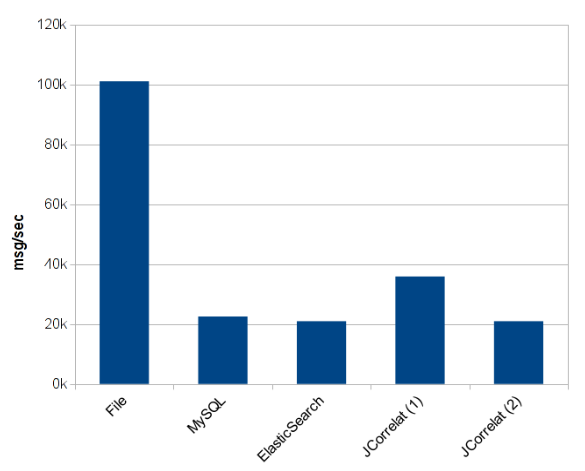
\includegraphics[scale=0.46]{img/benchmark}  
\end{figure}

Abbildung \ref{pic:benchmark} (\cite{reissmann}) zeigt die Ergebnisse eines Benchmarks 
über das gesamte Korrelationssystem hinweg.\\

\textbf{File} zeigt die Anzahl der Meldungen die normalisiert werden können, wenn die 
normalisierten Syslog-Meldungen lokal in Dateien geschrieben werden.\\

Die Balken \textbf{Mysql} und \textbf{ElasticSearch} demonstrieren die Anzahl der 
normalisierten Syslog-Meldungen, wenn diese direkt über \textit{rsyslog}-eigene Module in 
diese Datenbanken geschrieben werden. Dabei wird eine auf HTTP-basierende Schnittstelle 
verwendet.\\

Über 30.000 normalisierte Syslog-Meldungen (\textbf{JCorrelat (1)}) können hingegen mit 
\textit{JCorrelat} über die \textit{elasticsearch}-API direkt in \textit{elasticsearch} 
geschrieben werden, was die Differenz zum vorhergehenden Balken erklärt, da hier der 
HTTP-Verwaltungsaufwand entfällt.\\

Bei \textbf{JCorrelat (2)} wurde die Korrelationsfunktion aktiviert. Damit ist 
\textit{JCorrelat} genau so performant, als wenn die normalisierten Daten lediglich in 
eine Datenbank geschrieben würden.
